\section{What averaged bounds recover pointwise}
\label{sec:mean-pointwise}

The preceding reports establish two useful interfaces: reciprocal-scale
convexity for sparse sampling \cite{priorSampling}, and a positive-part
Mellin criterion that accepts averaged error bounds \cite{priorMean}.
This section combines them to quantify what those averages imply at
individual points. The resulting exponent is sharp even for positive,
uniformly bounded coefficients supported on the integers.

This is an additional synthesis within the inspected reports, not a claim
of priority for a general interpolation principle. Estimates from
$L^p$ to $L^\infty$ for semiconvex functions are part of the existing
literature; see Braga--Figalli--Moreira, Section~8, Proposition~8.2
\cite{BFM}. Here the one-sided statement, constants, and positive-measure
countermodel are proved directly.

\subsection{A local inequality with explicit constants}

Let $\mu$ be a positive locally finite Borel measure on $[1,\infty)$,
let $A\ge0$ and $c\in\R$, and put
\begin{equation}\label{eq:mpt-ramp}
 S(x)=\int_{[1,x]}\left(\frac1u-\frac1x\right)d\mu(u),
 \qquad R(x)=S(x)-A\log x-c \qquad (x\ge1).
\end{equation}
The source remainder has this form with $A=1/\varphi(q)$ and the
nonnegative prime-power weights of
\texttt{New/Reduction/Zeros/PrimeError.lean} \cite{source}.
For $p\ge1$ and $x\ge3/2$, define
\[
 M_p(x)=\frac1x\int_{2x/3}^{2x}\pos{R(y)}^p\,dy,
 \qquad h=\pos{R(x)},\qquad c_p=\frac{2^{2-p}}9.
\]

\begin{theorem}[Positive mass forced by a positive value]
\label{thm:mpt-local}
If $A>0$, then
\begin{equation}\label{eq:mpt-mass}
 M_p(x)\ge c_p h^p\min\left\{1,\sqrt{\frac{3h}{A}}\right\}.
\end{equation}
Consequently, with $D_p=9\cdot2^{p-2}$,
\begin{equation}\label{eq:mpt-point}
 h\le\max\left\{(D_pM_p(x))^{1/p},
 \left(D_p\sqrt{A/3}\,M_p(x)\right)^{1/(p+1/2)}\right\}.
\end{equation}
For $A=0$, one has $M_p(x)\ge c_p h^p$.
The constants are explicit, without a claim of optimality.
\end{theorem}

\begin{proof}
The function
\[
 H(t)=\int_{[1,\infty)}(u^{-1}-t)_+\,d\mu(u)
\]
is finite and convex for $t>0$, and equals $S(1/t)$ when
$0<t\le1$. Set $f(v)=R(x/v)$ for
$1/2\le v\le3/2$. Then $f(v)-A\log v$ is convex, so its
midpoint inequality gives
\begin{equation}\label{eq:mpt-midpoint}
 f(1-z)+f(1+z)\ge2f(1)+A\log(1-z^2),
 \qquad 0\le z\le1/2.
\end{equation}
The assertion is immediate if $h=0$. Otherwise $f(1)=h>0$.
The function $t\mapsto\pos{t}^p$ is convex and nondecreasing; hence
\[
 \pos{f(1-z)}^p+\pos{f(1+z)}^p
 \ge2\pos{h+(A/2)\log(1-z^2)}^p.
\]
Since $\log(1-z^2)\ge-4z^2/3$ for $0\le z\le1/2$, the right
side is at least $2(h/2)^p$ on $0\le z\le r$, where
\[
 r=\min\left\{\frac12,\sqrt{\frac{3h}{4A}}\right\}.
\]
The change of variables $y=x/v$ therefore yields
\[
 M_p(x)=\int_{1/2}^{3/2}\pos{f(v)}^p\frac{dv}{v^2}
 \ge\frac49\int_{1/2}^{3/2}\pos{f(v)}^p\,dv
 \ge\frac{8r}{9}(h/2)^p.
\]
This is \eqref{eq:mpt-mass}. Splitting at $h=A/3$ proves
\eqref{eq:mpt-point}. If $A=0$, use $r=1/2$ directly.
No differentiability of $R$ or $\mu$ is required.
\end{proof}

\begin{corollary}[Dyadic moments to pointwise values]
\label{cor:mpt-exponent}
Suppose $A>0$, $p\ge1$, and $\gamma>0$. If for every $\varepsilon>0$
\begin{equation}\label{eq:mpt-dyadic}
 \int_X^{2X}\pos{R(y)}^p\,dy
 \ll_\varepsilon X^{1-p\gamma+\varepsilon}
\end{equation}
for every sufficiently large dyadic $X$, then
\begin{equation}\label{eq:mpt-exponent}
 \pos{R(x)}\ll_\varepsilon
 x^{-2p\gamma/(2p+1)+\varepsilon}.
\end{equation}
\end{corollary}

\begin{proof}
Cover $[2x/3,2x]$ by a bounded number of dyadic intervals whose sizes
are comparable with $x$. Then
$M_p(x)\ll_\varepsilon x^{-p\gamma+\varepsilon}$.
Taking an exponent $\varepsilon<p\gamma$ first shows $M_p(x)\to0$.
Inequality~\eqref{eq:mpt-mass} forces $h\to0$, so its small-$h$
branch applies eventually. It gives \eqref{eq:mpt-exponent}, after
choosing the input $\varepsilon$ sufficiently small.
\end{proof}

At the square-root mean scale $\gamma=1/2$, this yields
\[
\begin{array}{c|c}
\text{averaged input}&\text{pointwise conclusion from positivity}\\ \hline
\displaystyle\int_X^{2X}\pos{R}\ll_\varepsilon X^{1/2+\varepsilon}
 &\pos{R(x)}\ll_\varepsilon x^{-1/3+\varepsilon}\\[2mm]
\displaystyle\int_X^{2X}\pos{R}^2\ll_\varepsilon X^\varepsilon
 &\pos{R(x)}\ll_\varepsilon x^{-2/5+\varepsilon}\\[2mm]
\displaystyle\int_X^{2X}\pos{R}^p\ll_\varepsilon X^{1-p/2+\varepsilon}
 &\pos{R(x)}\ll_\varepsilon x^{-p/(2p+1)+\varepsilon}.
\end{array}
\]

\begin{remark}[The analytic route does not incur this loss]
Under the meromorphic continuation and real-residue hypotheses,
the positive-part Mellin criterion of \cite{priorMean} already excludes
poles to the right of $1/2$ from each displayed input, using H\"older's
inequality when $p>1$. Recovering a pointwise estimate first would
unnecessarily weaken the zero-free conclusion. Theorem~\ref{thm:mpt-local}
instead gives a local certificate and identifies the precise limitation
of positivity alone. It does not provide a new arithmetic estimate.
\end{remark}

\subsection{Sharpness with bounded coefficients on integer support}

The following construction strengthens the earlier examples of narrow
positive spikes \cite{priorMean}: it retains the positive-ramp structure
and uniformly bounded integer-supported weights.

\begin{proposition}[Optimal exponent in the positive-ramp class]
\label{prop:mpt-sharp}
Fix $p\ge1$ and $0<\gamma<1$, and set
$\alpha=2p\gamma/(2p+1)$. There are positive coefficients $a_n$,
with $1/2\le a_n\le3/2$ for $n\ge2$ and
$\sum_{n\le x}a_n\sim x$, and a real constant $c_d$, such that
\[
 R_d(x)=\sum_{n\le x}a_n\left(\frac1n-\frac1x\right)-\log x-c_d
\]
satisfies \eqref{eq:mpt-dyadic} with $\varepsilon=0$, while
\[
 R_d(4^k)\sim(4^k)^{-\alpha}\qquad(k\to\infty).
\]
Thus the exponent in \eqref{eq:mpt-exponent} cannot be increased
for this class.
\end{proposition}

\begin{proof}
Let $X_k=4^k$, $h_k=X_k^{-\alpha}$, and
$L_k=10X_k\sqrt{h_k}$. Start at an integer $k_0$ large enough that
$h_k\le1/400$ for $k\ge k_0$. Define the compactly supported $C^2$
function
\[
 \psi(z)=\begin{cases}(1-z^2)^3,&|z|\le1,\\0,&|z|>1,\end{cases}
 \qquad
 R_c(x)=\sum_{k\ge k_0}h_k\psi\left(\frac{x-X_k}{L_k}\right).
\]
The supports are disjoint, because $L_k\le X_k/2$ and successive
centers have ratio four. The function and its first two derivatives
fit continuously at the support endpoints. Direct differentiation gives
\[
 \max|\psi'|=\frac{96}{25\sqrt5}<2,
 \qquad \max|\psi''|=6.
\]
Indeed $\psi''=-6+36z^2-30z^4$ on the support; its interior maximum
is $24/5$, and its minimum is $-6$.

Put $w(x)=1+(x^2R_c'(x))'$ and
$\mu_c=\delta_1+w(x)\,dx$ on $[1,\infty)$. On the $k$th support,
$x\le3X_k/2$, and therefore
\[
 |w(x)-1|
 \le\frac{6x^2h_k}{L_k^2}+\frac{4xh_k}{L_k}
 \le\frac{27}{200}+\frac35\sqrt{h_k}
 \le\frac{33}{200}<\frac12.
\]
Thus $1/2\le w\le3/2$. Integration gives
$\mu_c([1,x])=x+x^2R_c'(x)$. Differentiating the ramp sum and
comparing values at $1$ proves the exact identity
\begin{equation}\label{eq:mpt-continuous-id}
 S_{\mu_c}(x)-\log x=R_c(x).
\end{equation}
On each bump,
\begin{align*}
 \int R_c(x)^p\,dx
 &=h_k^pL_k\int_{-1}^1\psi(z)^p\,dz\\
 &=10\left(\int_{-1}^1\psi(z)^p\,dz\right)
 X_k^{1-\alpha(p+1/2)}
 =C_pX_k^{1-p\gamma}.
\end{align*}
Every dyadic interval meets at most two supports with comparable
centers. This proves the required mean bound for $R_c$; its peak
at $X_k$ is exactly $X_k^{-\alpha}$.

To obtain integer-supported weights, set
\[
 a_n=\mathbf1_{n=1}+\int_n^{n+1}w(u)\,du,
 \qquad
 c_d=\int_1^\infty w(u)
 \left(\frac1{\lfloor u\rfloor}-\frac1u\right)du.
\]
The last integral converges absolutely. The stated coefficient bounds
hold for $n\ge2$, and $3/2\le a_1\le5/2$.
For $N=\lfloor x\rfloor$, direct subtraction gives
\begin{align}
 R_d(x)-R_c(x)
 ={}&-\int_{N+1}^\infty w(u)
       \left(\frac1{\lfloor u\rfloor}-\frac1u\right)du\nonumber\\
 &+\int_x^{N+1}w(u)\left(\frac1u-\frac1x\right)du.
 \label{eq:mpt-discrete-id}
\end{align}
Both terms are nonpositive. For $x\ge2$, their absolute values sum to
at most $3/(2N)+3/(4x^2)\le4/x$. Hence
\begin{equation}\label{eq:mpt-discrete-error}
 0\le R_c(x)-R_d(x)\le4/x.
\end{equation}
It follows that $\pos{R_d}\le R_c$, preserving the mean bound.
Since $\alpha<1$, the peaks satisfy
$R_d(X_k)=X_k^{-\alpha}+O(X_k^{-1})\sim X_k^{-\alpha}$.
Finally, $x^2R_c'(x)=O(x\sqrt{h_k})=o(x)$ on the supports and
vanishes elsewhere. Thus $\mu_c([1,x])\sim x$; rounding intervals
changes this by $O(1)$, proving $\sum_{n\le x}a_n\sim x$.
\end{proof}

\begin{figure}[htbp]
 \centering
 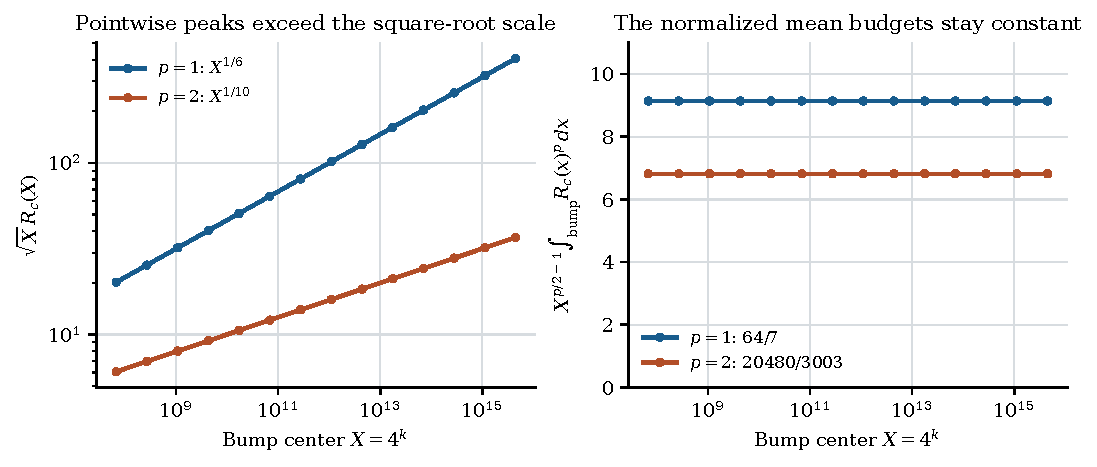
\includegraphics[width=\linewidth]{figures/mean_sharpness.pdf}
 \caption{The continuous sharpness models with $\gamma=1/2$.
 The normalized pointwise peaks grow, while their corresponding
 normalized moment budgets remain constant. Integer discretization
 changes the remainder by $O(1/x)$, preserving these asymptotics.
 These are synthetic positive weights, not prime data.}
 \label{fig:mpt-sharpness}
\end{figure}

The coefficients in Proposition~\ref{prop:mpt-sharp} satisfy a stronger
size bound than $a_n=O(\log n)$. They do not have prime-power support,
an Euler product, or an $L$-function functional equation. The example
therefore limits an abstract inference, without disproving any stronger
statement about actual primes.

\subsection{Compatibility with meromorphic continuation}

The countermodel also has the analytic properties relevant to the
mean criterion. This checks that the mean-to-pointwise gap is not
merely an artifact of a function lacking analytic continuation.

Write $(s)_j=s(s+1)\cdots(s+j-1)$, with $(s)_0=1$, and define
\[
 J_m(s)=\frac{(s)_{2m}}{(2m)!}
       \int_{-1}^1z^{2m}\psi(z)\,dz.
\]
Expanding $(1+\delta z)^{-s}$, where
$\delta=10X_k^{-\alpha/2}\le1/2$, and using the evenness of $\psi$
gives, initially far to the right,
\begin{equation}\label{eq:mpt-meromorphic}
 F_c(s)=\int_1^\infty R_c(x)x^{-s}\,dx
 =10\sum_{m\ge0}100^mJ_m(s)
 \frac{4^{k_0(1-s-\alpha(m+3/2))}}
      {1-4^{1-s-\alpha(m+3/2)}}.
\end{equation}
The series defines a meromorphic function on $\C$. Indeed, on any
compact set avoiding the displayed poles, its sufficiently late terms
are bounded by a polynomial in $m$ times
$(100\cdot4^{-k_0\alpha})^m$, and this geometric ratio is at most
$1/4$. Only finitely many remaining terms need separate consideration.
Possible poles are simple and lie at
\[
 s=1-\alpha(m+3/2)+\frac{2\pi i n}{\log4},
 \qquad m\ge0,\ n\in\mathbb Z.
\]
At a positive real pole $u=1-\alpha(m+3/2)$ the residue is
$10\cdot100^mJ_m(u)/\log4>0$. The rightmost line is
\[
 \Re s=1-3\alpha/2
 =1-\frac{3p\gamma}{2p+1}\le1-\gamma,
\]
with equality when $p=1$.
By \eqref{eq:mpt-discrete-error}, $F_d-F_c$ is holomorphic on
$\Re s>0$. Thus the discrete model has the same possible poles and
residues in that half-plane. Global meromorphic continuation of $F_d$
is not asserted.

At $\gamma=1/2$, these models satisfy the sharp mean budget and have
no pole to the right of $1/2$, yet their peaks decay only as
$x^{-p/(2p+1)}$. The usual sharper pointwise conclusions for arithmetic
$L$-functions require their additional structure and growth estimates.
For a proposed determinant transfer, the practical instruction is to
apply the mean criterion directly when it is available, while using
Theorem~\ref{thm:mpt-local} for finite-window or pointwise diagnostics.
